\chapter{Program Design} \label{chp:program}
\section{Implementing the SCP Framework}

The SCP framework has been implemented in \texttt{Python 3} as series of modules which follow strong object-oriented programming principles which support simple extensions and revisions. This implementation is used to demonstrate the practical approaches to generating and evaluating SCPs; and to model a series of cognitive tasks for which empirical results already exist. The library containing this implementation and its associated documentation is available at \href{https://github.com/AxelInd/SCP_Implementation}{github.com/AxelInd/SCP\_Implementation}.

At present, concrete implementations for epistemic state structures and cognitive operation formulations related to propositional logic, the WCS, and Reiter's default logic are provided.

\section{A Modular Programming Approach}
% talk about each 
The principle of modular programming is followed in this implementation to the greatest extent possible, thus maximising the ease of modification and upkeep for the program. Figure~\ref{fig:scpClassDiagram} provides a simplified class diagram to explain how the major components of the system relate to one another.

\subsection{Most Important Modules}


\begin{sidewaysfigure}
\centering 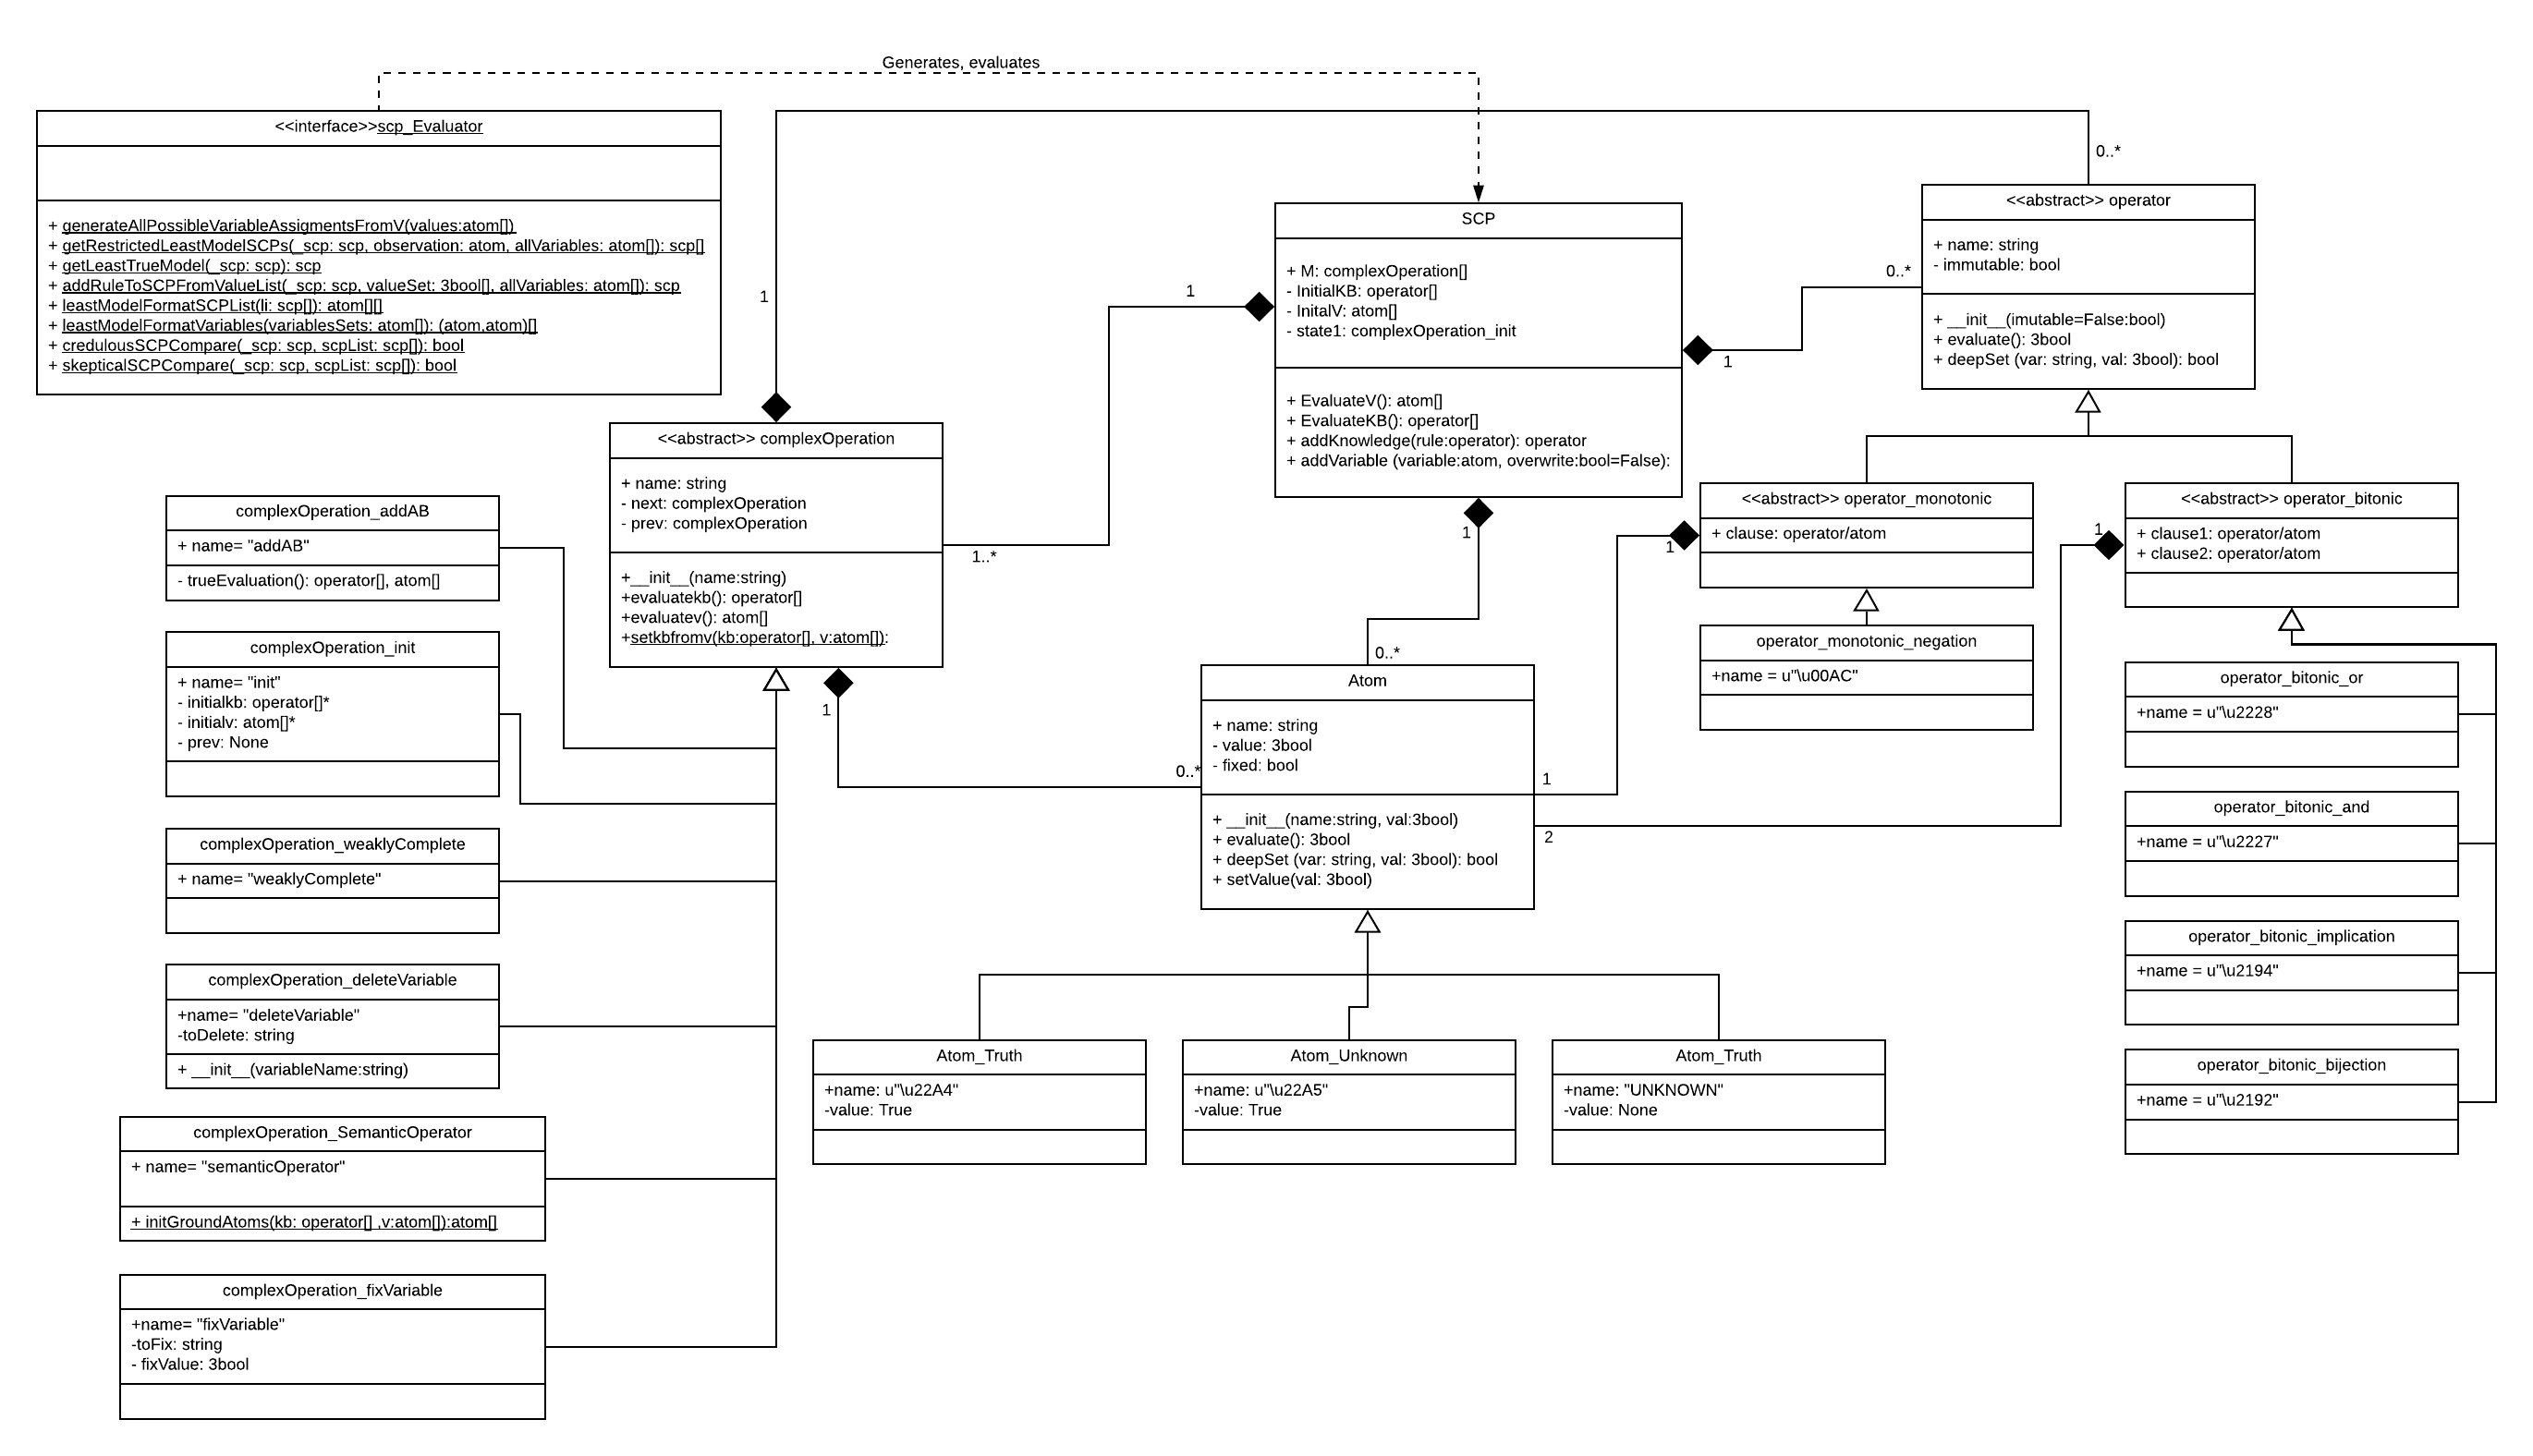
\includegraphics[width=0.75 \linewidth]{scpClassDiagram}
\caption{Class diagram for the implementation of the SCP Framework.}
\label{fig:scpClassDiagram}
\end{sidewaysfigure}


\begin{itemize}
\item $\texttt{SCPFramework/basicLogic}$: an implementation of basic two and three-valued logic.
\item $\texttt{SCPFramework/SCP\_Task}$: implements both the SCP Task ($\Pi$) object and a search function for generating SCPs which meet the given goals.
\item $\texttt{SCPFramework/CTM}$: implements the CTM $\pi$ and defines the $J[p,m]$ application of a cognitive operation to an input state point
\item $\texttt{SCPFramework/CognitiveOperations}$: defines the set of cognitive operations as well as the their input and output parameters.
\item $\texttt{SCPFramework/StatePointOperations}$: defines $f(\pi) \models_\text{strict} \gamma$ and $f(\pi) \models_\text{weak} \gamma$ determining if a given SCP meets a given set of output criteria.
\item $\texttt{SCPFramework/truthTables}$: a set of truth tables for each operator defined in \texttt{basicLogic}.
\item $\texttt{ScoringAlgorithms/SCP\_scoring}$: an implementation of the Needleman-Wunsch Algorithm for SCPs described in Chapter~\ref{chp:comparing}
\item $\texttt{ScoringAlgorithms/SCP\_scoring\_improved}$: an implementation of the extended Needleman Wunsch Algorithm for SCPs described in Chapter~\ref{chp:comparing}
\end{itemize}

\subsection{Program Flow}
\begin{figure}
\centering 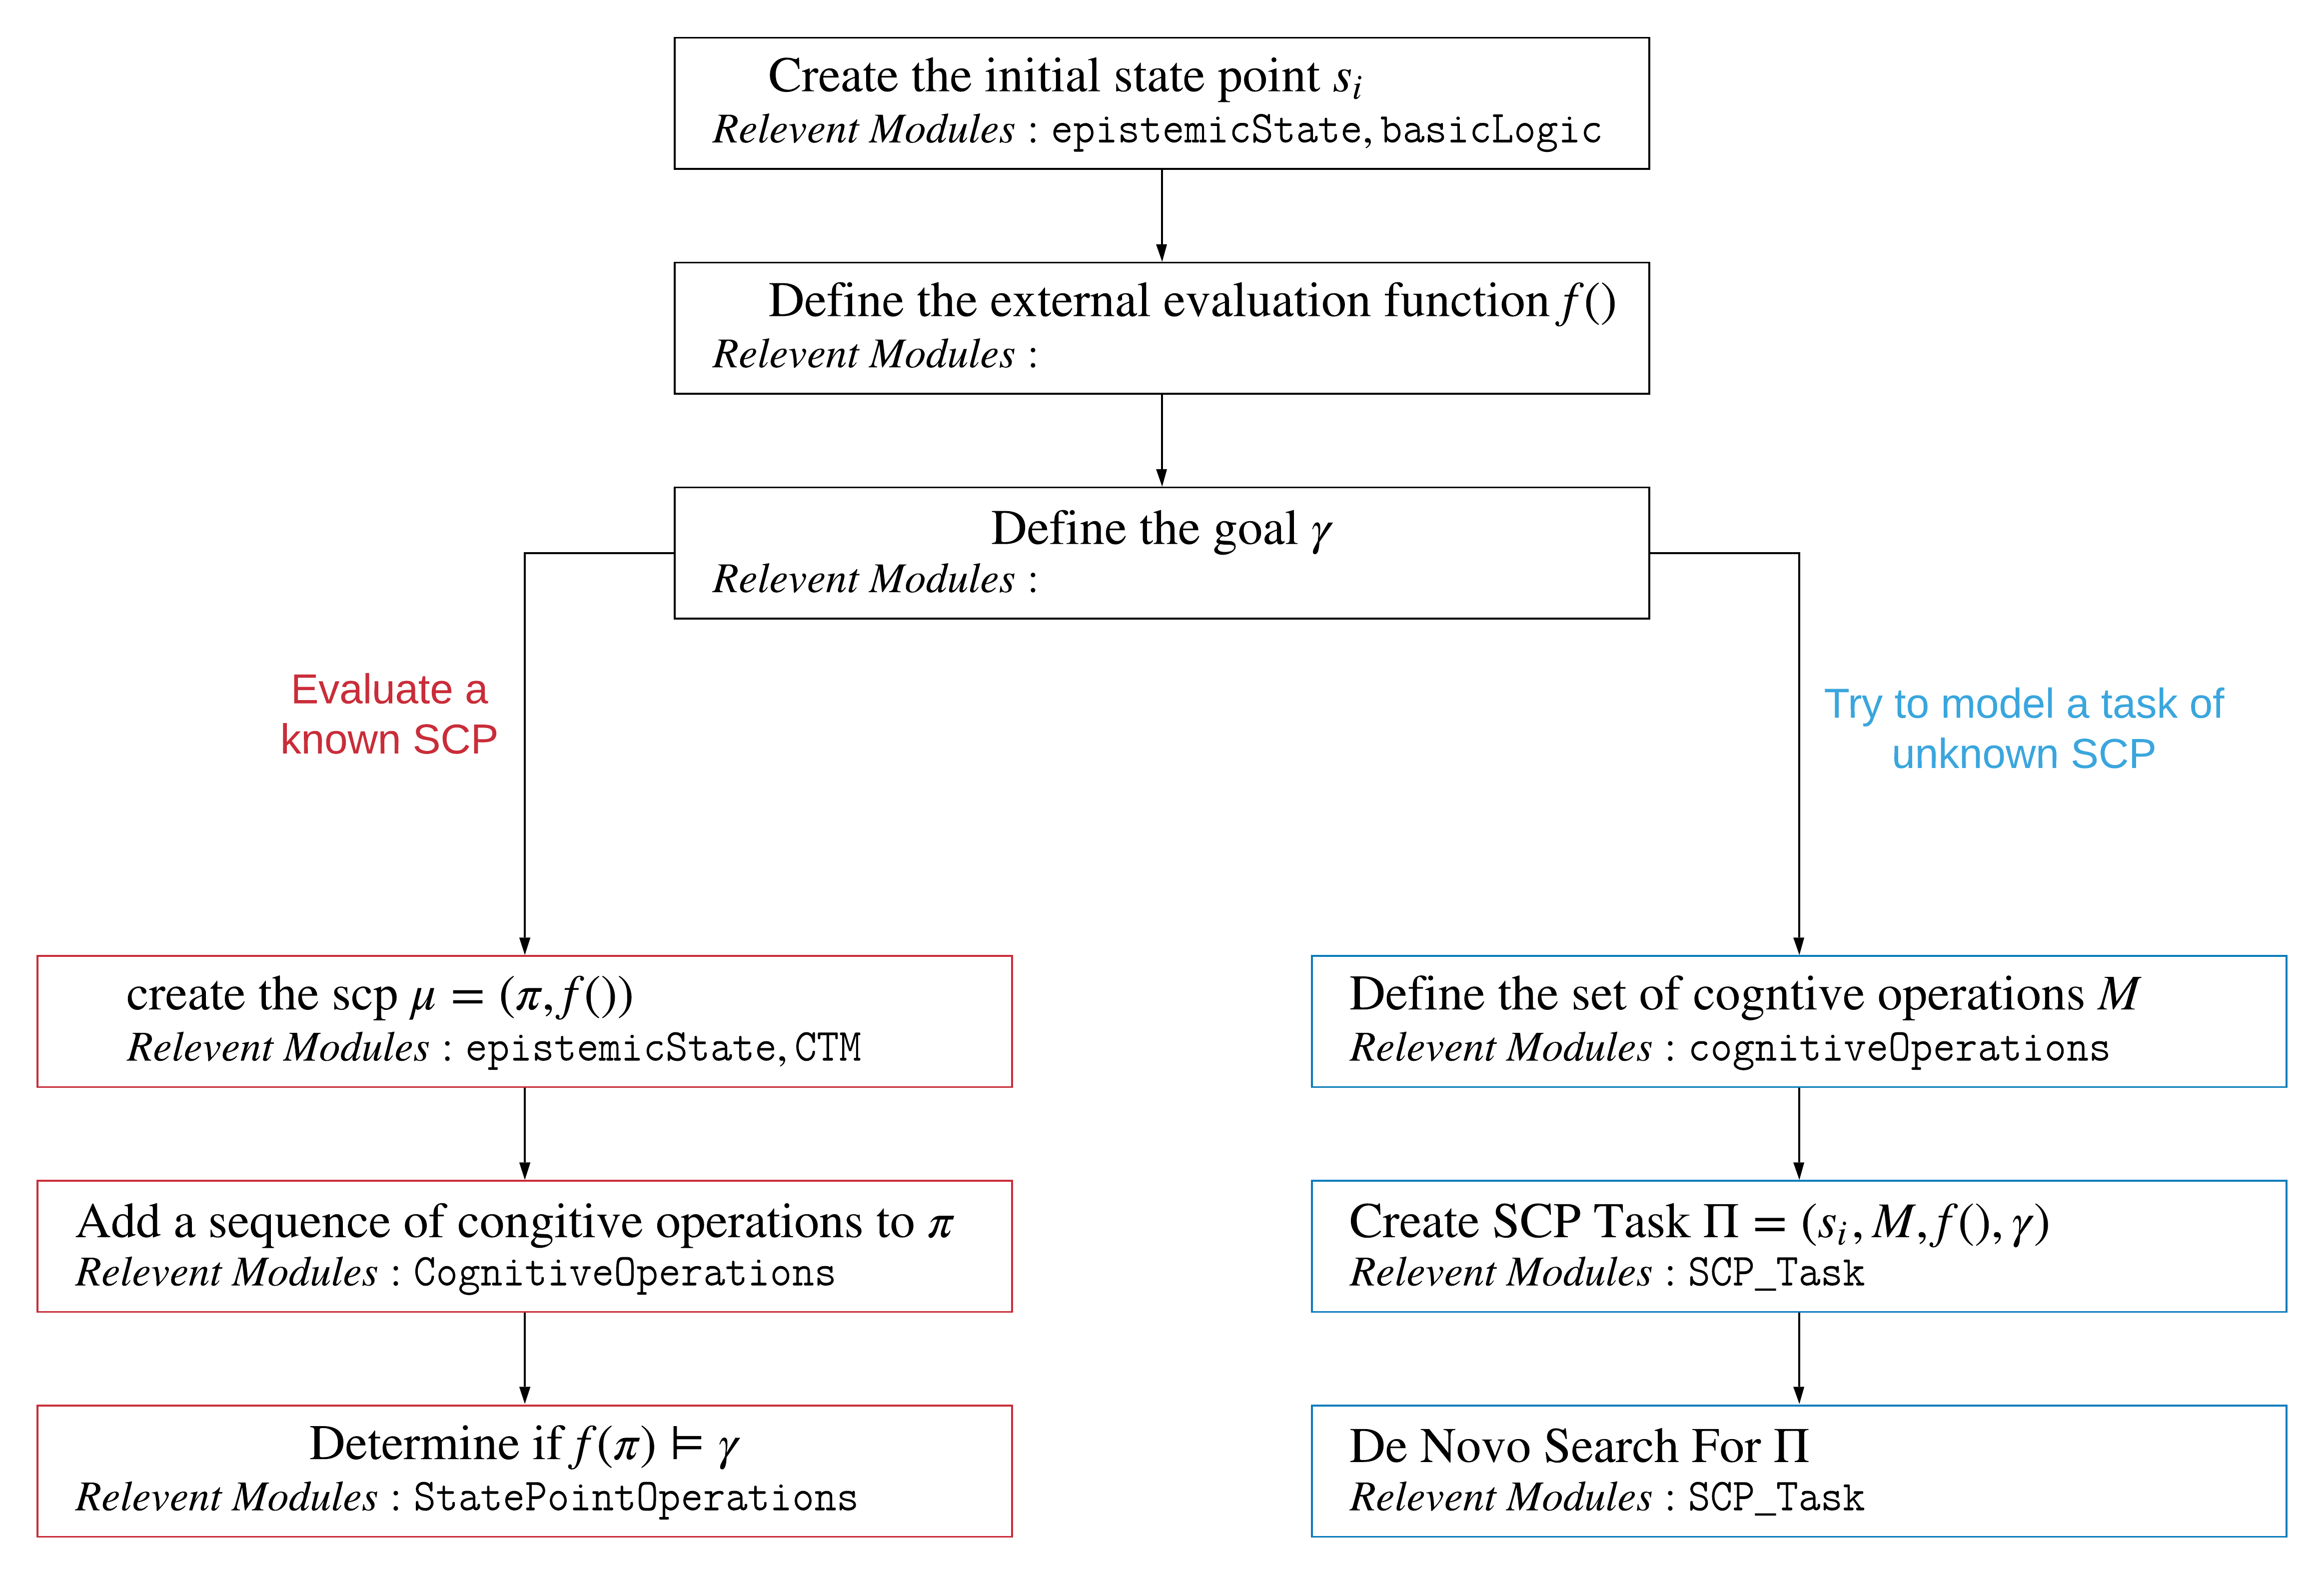
\includegraphics[width=\linewidth]{SCP_Use_Cases}
\caption{Two use cases for the implementation of the SCP framework}
\label{fig:SCP_Use_Cases}
\end{figure}



Diagram~\ref{fig:SCP_Use_Cases} illustrates the basic programmatic flow used to model either a known SCP or known empirical result set using the SCP Framework. In the appendix, Figure~\ref{fig:sup_snippet} provides a code snippet to show exactly how the general case of the Suppression Task is modelled in the SCP framework.



\subsection{Modelled Experiments}
\begin{itemize}
\item \texttt{example\_wcs\_suppressionTask.py}: models the Suppression Task as discussed in Chapter~\ref{chp:model}.
\item \texttt{example\_wcs\_wst.py}: models the Wason Selection Task as discussed in Chapter~\ref{chp:model}.
\item \texttt{example\_default\_various.py}: models of the Suppression Task, Penguin Case, and Nixon Diamond implemented with a default-logic capable SCP.
\end{itemize}

\section{External Framework Integration}
At present work is ongoing to integrate the SCP framework with the \texttt{CCOBRA} \citep{ccobra} cognitive modelling environment.













